\documentclass{sigchi}

% Use this section to set the ACM copyright statement (e.g. for
% preprints).  Consult the conference website for the camera-ready
% copyright statement.

% Copyright



% ISBN
%\isbn{123-4567-24-567/08/06}
%Price
%\acmPrice{\$15.00}

% Use this command to override the default ACM copyright statement
% (e.g. for preprints).  Consult the conference website for the
% camera-ready copyright statement.

%% HOW TO OVERRIDE THE DEFAULT COPYRIGHT STRIP --
%% Please note you need to make sure the copy for your specific
%% license is used here!
% \toappear{
% Permission to make digital or hard copies of all or part of this work
% for personal or classroom use is granted without fee provided that
% copies are not made or distributed for profit or commercial advantage
% and that copies bear this notice and the full citation on the first
% page. Copyrights for components of this work owned by others than ACM
% must be honored. Abstracting with credit is permitted. To copy
% otherwise, or republish, to post on servers or to redistribute to
% lists, requires prior specific permission and/or a fee. Request
% permissions from \href{mailto:Permissions@acm.org}{Permissions@acm.org}. \\
% \emph{CHI '16},  May 07--12, 2016, San Jose, CA, USA \\
% ACM xxx-x-xxxx-xxxx-x/xx/xx\ldots \$15.00 \\
% DOI: \url{http://dx.doi.org/xx.xxxx/xxxxxxx.xxxxxxx}
% }

% Arabic page numbers for submission.  Remove this line to eliminate
% page numbers for the camera ready copy
% \pagenumbering{arabic}

% Load basic packages
\usepackage{balance}       % to better equalize the last page
\usepackage{graphics}      % for EPS, load graphicx instead 
\usepackage[T1]{fontenc}   % for umlauts and other diaeresis
\usepackage{txfonts}
\usepackage{mathptmx}
\usepackage[pdflang={en-US},pdftex]{hyperref}
\usepackage{color}
\usepackage{booktabs}
\usepackage{textcomp}

% Some optional stuff you might like/need.
\usepackage{microtype}        % Improved Tracking and Kerning
% \usepackage[all]{hypcap}    % Fixes bug in hyperref caption linking
\usepackage{ccicons}          % Cite your images correctly!
% \usepackage[utf8]{inputenc} % for a UTF8 editor only

% If you want to use todo notes, marginpars etc. during creation of
% your draft document, you have to enable the "chi_draft" option for
% the document class. To do this, change the very first line to:
% "\documentclass[chi_draft]{sigchi}". You can then place todo notes
% by using the "\todo{...}"  command. Make sure to disable the draft
% option again before submitting your final document.
\usepackage{todonotes}

% Paper metadata (use plain text, for PDF inclusion and later
% re-using, if desired).  Use \emtpyauthor when submitting for review
% so you remain anonymous.
\def\plaintitle{A Secure, Privacy-Preserving IoT Middleware Using Intel SGX }
\def\plainauthor{First Author, Second Author, Third Author,
  Fourth Author, Fifth Author, Sixth Author}
\def\emptyauthor{}
\def\plainkeywords{IoT Middleware; Privacy-Aware Computing; Security; Trusted Execution Environments; Intel SGX }
\def\plaingeneralterms{Documentation, Standardization}

% llt: Define a global style for URLs, rather that the default one
\makeatletter
\def\url@leostyle{%
  \@ifundefined{selectfont}{
    \def\UrlFont{\sf}
  }{
    \def\UrlFont{\small\bf\ttfamily}
  }}
\makeatother
\urlstyle{leo}

% To make various LaTeX processors do the right thing with page size.
\def\pprw{8.5in}
\def\pprh{11in}
\special{papersize=\pprw,\pprh}
\setlength{\paperwidth}{\pprw}
\setlength{\paperheight}{\pprh}
\setlength{\pdfpagewidth}{\pprw}
\setlength{\pdfpageheight}{\pprh}

% Make sure hyperref comes last of your loaded packages, to give it a
% fighting chance of not being over-written, since its job is to
% redefine many LaTeX commands.
\definecolor{linkColor}{RGB}{6,125,233}
\hypersetup{%
  pdftitle={\plaintitle},
% Use \plainauthor for final version.
%  pdfauthor={\plainauthor},
  pdfauthor={\emptyauthor},
  pdfkeywords={\plainkeywords},
  pdfdisplaydoctitle=true, % For Accessibility
  bookmarksnumbered,
  pdfstartview={FitH},
  colorlinks,
  citecolor=black,
  filecolor=black,
  linkcolor=black,
  urlcolor=linkColor,
  breaklinks=true,
  hypertexnames=false
}

% create a shortcut to typeset table headings
% \newcommand\tabhead[1]{\small\textbf{#1}}

% End of preamble. Here it comes the document.
\begin{document}
\CopyrightYear{2017} 
\setcopyright{rightsretained} 
\conferenceinfo{IoT '17}{October 22--25, 2017, Linz, Austria}\isbn{978-1-4503-5318-2/17/10}
\doi{https://doi.org/10.1145/3131542.3140258}

\title{\plaintitle}

\numberofauthors{3}
\author{%
  \alignauthor{Pascal Gremaud\\
    \affaddr{University of Fribourg}\\
    \affaddr{Fribourg, Switzerland}\\
    \email{pascal.gremaud@unifr.ch}}\\
  \alignauthor{Arnaud Durand\\
    \affaddr{University of Fribourg}\\
    \affaddr{Fribourg, Switzerland}\\
    \email{arnaud.durand@unifr.ch}}\\
  \alignauthor{Jacques Pasquier\\
    \affaddr{University of Fribourg}\\
    \affaddr{Fribourg, Switzerland}\\
    \email{jacques.pasquier@unifr.ch}}\\
}

\maketitle

\begin{abstract}

With Internet of Things (IoT) middleware solutions moving towards cloud computing, the problems of trust in cloud platforms and data privacy need to be solved. The emergence of Trusted Execution Environments (TEEs) opens new perspectives to increase security in cloud applications. We propose a privacy-preserving IoT middleware, using Intel Software Guard Extensions (SGX) to create a secure system on untrusted platforms. An encrypted index is used as a database and communication with the application is protected using asymmetric encryption. This set of measures allows our system to process events in an orchestration engine without revealing data to the hosting cloud platform.

\end{abstract}

\category{D.2.11}{Software Architectures}{Information hiding} \category{E.3}{Data Encryption}{Public key cryptosystems}

\keywords{\plainkeywords}

\section{Introduction}

The constant growth of the IoT introduced a set of challenges, several important ones being related to security. While most of them are being addressed, the privacy subdomain still suffers from multiple unsolved ones. A critical issue is the fact that any IoT middleware performing data processing automatically requires access to these data. As Yan et al. observed, "[...] IoT services are based on data process, analysis and mining. This fact actually greatly intrudes user privacy" \cite{yan_trust_survey}. As cloud computing is seen as a convenient solution for IoT middlewares, one can only assume the trustworthiness of the hosting platform regarding application data, without being given any actual proof of it. However, trust is not sufficient in this context and it is widely accepted that more research is needed on this topic \cite{yan_trust_survey}\cite{sicari_privacy_survey}\cite{botta_survey}. To approach this problem, limited processing on encrypted data can be achieved using homomorphic encryption. Talos \cite{shafagh_talos} is a privacy-preserving system storing Things data in a cloud database and allowing queries on encrypted data. While it solves the privacy issue, this system is not able to run an orchestration engine in the cloud itself and thus relies on clients for handling the application logic. 

Since the last few years, several solutions to trust issues have been presented in the form of TEEs. Namely, Intel added a set of CPU instructions called SGX to their processors based on Skylake microarchitecture. These new instructions allow the creation of so-called enclaves, consisting of encrypted memory regions. The code and data inside an enclave are protected and cannot be accessed by any other processes, independently of their privilege level. This new technology enables secure computing on untrusted, remote platforms. Examples of using SGX to protect data execution include VC3 \cite{schuster_vc3}, a secure system for distributed MapReduce computations. The IoT middleware we propose uses SGX technology as a solution to privacy issues inherent to cloud computing.

\section{System Architecture Overview}


\begin{figure}
\centering
  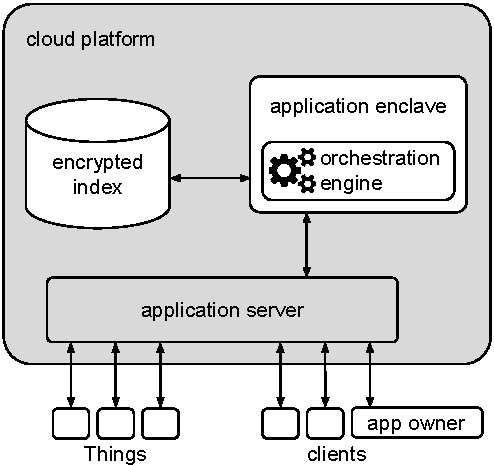
\includegraphics[width=0.8\columnwidth]{figures/system_pdf}
  \caption{General architecture of the system. The grey area corresponds to untrusted components. }~\label{fig:architecture}
\end{figure}

The components of our system architecture are shown in Fig.~\ref{fig:architecture}. The cloud platform hosts the application and is an untrusted part of the system. The enclave inside it contains an orchestration engine to interact with the Things and clients, which code and data are not accessible by the cloud platform. SGX was not designed to efficiently protect large portions of memory, this is why an encrypted index outside the enclave is used as a database. Its encryption key is provisioned by the application owner and stored inside the enclave. As a consequence, the index itself is considered trusted. Several secure indexes such as CryptDB \cite{popa_cryptdb} allow query execution over encrypted data and can be used to increase time performance for data retrieval. The index contains Things data as well as the orchestration engine data, as we do not necessarily considerate the application enclave as a long-lived component. This is also the reason why no information is stored solely inside the enclave. An application server is used as an interface between the application and the outside world. Being an untrusted component, all of the messages payloads it processes are encrypted. Things communicate with the application via the application server and thus need to be able to encrypt and decrypt messages they send and receive. Clients have the same role as Things while being oriented towards data consumption rather than data production. Finally, the application owner is a particular client whose main task is to instantiate the application and to create and manage the orchestration engine rules.

%In order to ensure the system is secure, communications between the application server, the %clients and the Things all asymetric encryption for message payloads.

\section{Secure Initialization and Communication}

All participants (the application, Things, and clients) use asymmetric encryption to communicate. The system itself is protocol-agnostic, most messaging protocols with asymmetric encryption support are suitable for implementation. Once the enclave is created by the untrusted platform, a remote attestation procedure is started using an attestation service provided by Intel, proving to the application owner that he is communicating with a genuine enclave containing the expected application code. In parallel, the untrusted platform transmits the public key of the application owner to the enclave. On attestation success, the application owner can establish a secure communication with the enclave and verify that he has been registered in it. The last step is the enclave receiving the key of the encrypted index from the application owner. At this point, the three essential trusted components have been initialized and the system is operational.

Once the setup has been completed, the concept of trusted and untrusted components is transparent to the participants. The application owner registers both Things and clients to the application. The public key of each of the registered participants is stored in the index and the public key of the enclave is shared with them. Finally, the application owner uploads the application logic (i.e. the orchestration engine rules) to the enclave. Alternatively, the entire index can be securely uploaded via the untrusted application server if an application is migrated from another platform. 

At this point, it is necessary to understand that some data cannot be protected from the untrusted components. While the content of exchanged messages is inaccessible, it is still possible to infer information by analyzing the frequency of the messages, as well as the identity of the clients or Things sending (or receiving) them. One can, for instance, deduce a link between a Thing and a client if a message is systematically sent to a client after one is sent to the platform from a given Thing. Analyzing the message frequency, the untrusted components could also deduce whether a Thing is a simple logger using fixed time intervals or is communicating based on events. Even when considering such scenarios, the attack surface remains limited and the actual data is never revealed.


\section{Conclusion and Future Work}
In this poster, we propose a secure, privacy-preserving IoT middleware using Intel SGX. By enabling secure computation in untrusted environments, such a system can solve important security issues inherent to cloud computing. More generally, TEEs offer impressive, new solutions to solve problems related to privacy and security in general. 

A first prototype of the proposed architecture is being implemented with the Intel SGX Software Development Kit (SDK) for Linux, in conjunction with web technologies---Restful Web Services, JSON Web Encryption (JWE)---and shows the feasibility of the project. As next steps an extensive security analysis of the system would highlight its strengths and weaknesses and could open the way to other similar approaches for IoT middlewares. We will also produce performance tests to ensure that the overhead introduced by both SGX and the systematically encrypted communications does not prevent the system from being used as an actual middleware solution.



% BALANCE COLUMNS
\balance{}

% REFERENCES FORMAT
% References must be the same font size as other body text.
\bibliographystyle{SIGCHI-Reference-Format}
\bibliography{sample}

\end{document}

%%% Local Variables:
%%% mode: latex
%%% TeX-master: t
%%% End:
